\documentclass[a4paper]{article}

\usepackage[utf8]{inputenc}
\usepackage[T1]{fontenc}
\usepackage{textcomp}
\usepackage[italian]{babel}
\usepackage{amsmath, amssymb}
\usepackage{listings}
\usepackage{graphicx}
\usepackage{hyperref}

\title{Relazione di Laboratorio 1 - Pendolo Fisico}
\author{Walhout Francesco - Iallorenzi Michele}

\begin{document}
    \maketitle
    
    \section{Introduzione}
    Il Pendolo Fisico, anche chiamato Pendolo Composto, è un pendolo che, a differenza del classico pendolo con una massa e filo ideale (inestensibile e privo di massa) attaccato al punto di sospensione, ha una massa del filo non trascurabile. Si può chiamare pendolo fisico un qualsiasi oggetto, attaccato ad un punto di sospensione, libero di oscillare. Esempi più classici di pendoli fisici sono delle aste di un materiale con densità costante. Nel nostro caso avremo un'asta metallica forata, che oscilla su uno dei fori (punti di sospensione). Lo scopo dell'esperimento è quello di misurare le oscillazioni del pendolo, in funzione della distanza tra centro di massa e punto di sospensione, e confrontare i dati con un modello matematico, verificando che questo descriva al meglio il fenomeno fisico con il Test del $\chi^2$.
    
    \section{Esperienza}
    
    \subsection{Strumenti}
    \begin{itemize}
        \item Un'asta metallica forata.
        \item Un supporto di sospensione.
        \item Cronometro (risoluzione $0.01 [s]$)
        \item Metro a nastro (risoluzione $1 [mm]$)
        \item Calibro ventesimale (risoluzione $0.05 [mm]$)
    \end{itemize}
    
    \subsection{Misurazione}
    L'esperimento prevede di misurare 10 oscillazioni per 5 volte, fatte sui 10 punti di sospensione. Per misurare un oscillazione completa, partendo da una certa ampiezza iniziale del pendolo, è necessario contare gli istanti in cui il pendolo si ferma completamente, quindi assicurandosi che le oscillazioni siano complete.
    Qui si possono trovare due difficoltà:
    \begin{enumerate}
        \item non si ferma il cronometro nell'istante in cui l'energia cinetica del pendolo è 0 (quindi l'istante in cui si completa un oscillazione), in questo modo si possono fare degli errori sul centesimo di secondo;
        \item le oscillazioni del pendolo non sono omogenee dato che può oscillare sul suo supporto, quindi non è perfettamente vincolato ad oscillare lungo un piano.
    \end{enumerate}
    
    Risolvere il secondo problema è semplice, bisogna aspettare qualche secondo, in modo tale che il pendolo compia delle oscillazioni omogenee (sviluppate solo su un piano); per il primo problema ci è stata data una soluzione dal Prof. Giudici. La sua soluzione si appoggia ad una ricerca condotta dall'Università di Pisa che dimostra che una semplice azione è in grado di sincronizzare i ritmi della visione, quindi è possibile sincronizzare il nostro cervello con le oscillazioni del pendolo, eliminando così gli errori sul centesimo di secondo e riuscendo a fermare il cronometro nell'istante dell'oscillazione finale. Quindi per risolvere questo primo problema è necessario, dopo aver aspettato che il pendolo si stabilizzi, osservare con attenzione il pendolo per qualche secondo e poi far partire il tempo.
    
    \section{Calcoli}
        Per iniziare i calcoli, definiamo il Momento della Forza di Gravità, che per un qualsiasi pendolo fisico (un qualsiasi oggetto attaccato ad un punto di sospensione, posto a distanza $D$ dal centro di massa, libero di oscillare), vale:
        \begin{equation}\label{eq:1}
            \vec{M_0} = \vec{P} \wedge \vec{d} = m g D sin\theta
        \end{equation}
        Per semplificare i calcoli, è possibile utilizzare questa nozione di Analisi sulle serie di Taylor, che mi dice che: $\sin(\theta) \sim \theta$. Di seguito allegheremo un immagine per giustificare questa approssimazione.
        
        \begin{figure}
            \centering
            \fbox{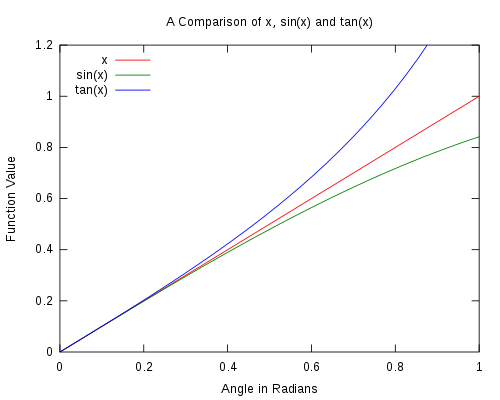
\includegraphics[width=.8\textwidth, height=.6\textheight, keepaspectratio]{extra/Small_angle_compair_odd.svg.png}}
            \caption{Approssimazione di Taylor sin(x)}
            \label{fig:my_label}
        \end{figure}
        
        Escludendo la funzione tangente (funzione in blu), possiamo notare che, nei primi 0.2 radianti (circa 11.5°) le due funzioni si sovrappongono. Infatti se calcoliamo il seno in 0.2 radianti:
        \begin{equation*}
            sin(0.2) = 1.9936 \sim 0.2
        \end{equation*}
        Dato che le differenze si possono incontrare alla millesima cifra, possiamo affermare che per oscillazioni che vanno sotto agli 11.5° (circa), si può scrivere la relazione \ref{eq:1} come:
        \begin{equation*}
            M_0 = - m g D \theta
        \end{equation*}
        Introduciamo la Seconda Equazione Cardinale e riscriviamola ricordando che  si può scrivere utilizzando il Momento di Inerzia: $L_0 = \omega I = \frac{d\theta}{dt}$.
        \begin{equation*}
            M_0 = \frac{dL_0}{dt} = I \frac{d^2\theta}{dt^2} = - m g d \theta
        \end{equation*}
        \begin{equation*}
            \frac{d^2\theta}{dt^2} + \frac{m g D \theta}{I} = 0
        \end{equation*}
        Risolvendo questa equazione differenziale è possibile trovare il periodo del pendolo:
        \begin{equation*}
            \omega_0 = \sqrt{\frac{mgD}{I}}
        \end{equation*}
        \begin{equation*}
            T_0 = \frac{2\pi}{\omega_0} = 2\pi \sqrt{\frac{mgD}{I}}
        \end{equation*}
        Il momento di inerzia si può calcolare attraverso il Teorema di Huygens-Steiner. Per un'asta con densità omogenea, rispetto ad una distanza d (tra P e centro di massa) è:
        \begin{equation*}
            I = I_{cm} + m D^2 = \frac{ml^2}{12} + md^2
        \end{equation*}
        Infine possiamo riscrivere il periodo (in funzione della distanza) come:
        \begin{equation}
            T(d) = 2\pi \sqrt{\frac{l^2/12 + D^2}{gD}}
        \end{equation}
        Un importate considerazione da fare è che il quadrato del periodo è inversamente proporzionale alla lunghezza d (distanza tra P e centro di massa) $ T^2 \propto D^{-1}$, questo vuol dire che ci aspettiamo un andamento iperbolico delle misure del periodo del pendolo in funzione della distanza, non ci resta che verificare quello che abbiamo appena detto.
        
    
    \section{Elaborazione dei dati}
    
    \subsection{Grafico}
        Il codice scritto in Python prende in input i tempi medi riportati nell'ultima riga della tabella \ref{tab:dati}, che cambiano in base alla distanza dal punto di sospensione, per poi restituire in output un grafico che descriva l'andamento dei tempi che, secondo i calcoli matematici, sono inversamente proporzionali alla distanza del pendolo. Una volta ricavato il grafico, per verificare che il modello è adeguato al fenomeno fisico, si fa un "Test del $\chi^2$ ".
    
    \subsection{Test del $\chi^2$}
        ...

    \section{Codice}
    
    \begin{lstlisting}[language=Python, caption=Codice]
        ...
    \end{lstlisting}
    
    \section{Conclusioni}
        Come si può chiaramente vedere dal grafico, i dati che sono stati riportati seguono un andamento iperbolico ed il test del $\chi^2$ restituisce un valore molto vicino ... Concludiamo che il modello descrive adeguatamente il fenomeno fisico.
        
    \section*{Dati}
    \begin{table}[h!]
        \centering
        \begin{tabular}{|c|c|c|c|c|c|c|c|c|c||c|}
             \hline
             1 & 2 & 3 & 4 & 5 & 6 & 7 & 8 & 9 & 10 & \\ [0.3ex]
             \hline\hline
             16.41 & 15.67 & 15.36 & 16.71 & 22.73 & 38.74 & 18.43 & 15.84 & 15.46 & 15.86 & \\
             16.32 & 15.51 & 15.60 & 16.65 & 22.44 & 38.45 & 18.42 & 15.93 & 15.75 & 15.97 & \\
             16.11 & 15.73 & 15.37 & 16.68 & 22.88 & 38.46 & 18.57 & 15.68 & 15.53 & 16.18 & \\
             16.43 & 15.37 & 15.61 & 16.76 & 22.59 & 38.79 & 18.39 & 15.96 & 15.44 & 15.93 & \\
             16.13 & 15.64 & 15.27 & 16.47 & 22.78 & 38.89 & 18.48 & 15.70 & 15.49 & 16.18 & \\
             \hline
             16.28 & 15.58 & 15.44 & 16.65 & 22.68 & 38.67 & 18.46 & 15.82 & 15.53 & 16.02 & Medie\\ 
             \hline
        \end{tabular}
        \caption{Dati sperimentali}
        \label{tab:dati}
    \end{table}
    
    \section*{Bibliografia}
        Ricerca sulla "Sincronizzazione sensori-motoria":\hyperbaseurl{https://www.unipi.it/index.php/news/item/21234-i-ritmi-del-cervello-per-la-sincronizzazione-sensori-motoria-l-azione-batte-il-tempo-della-percezione}
        Immagine sull'approssimazione per angoli piccoli:\hyperbaseurl{https://it.wikipedia.org/wiki/Approssimazione_per_angoli_piccoli}
    

\end{document}
